\section{Stream Design Anti-Patterns}
\label{sec:anti-pattern}
This elaborates on the anti-patterns we elicited through self-ethnography. These anti-patterns are elaborated further within OSTIA to allow for their detection during streaming topology inference analysis.

\subsection{Multi-Anchoring}
In order to guarantee fault-tolerant stream processing, tuples processed by bolts needs to be anchored with the unique id of the bolt and be passed to multiple ackers int he topology. Therefore, ackers can keep track of tuples in the topology.

\begin{figure}[H]
	\begin{center}
		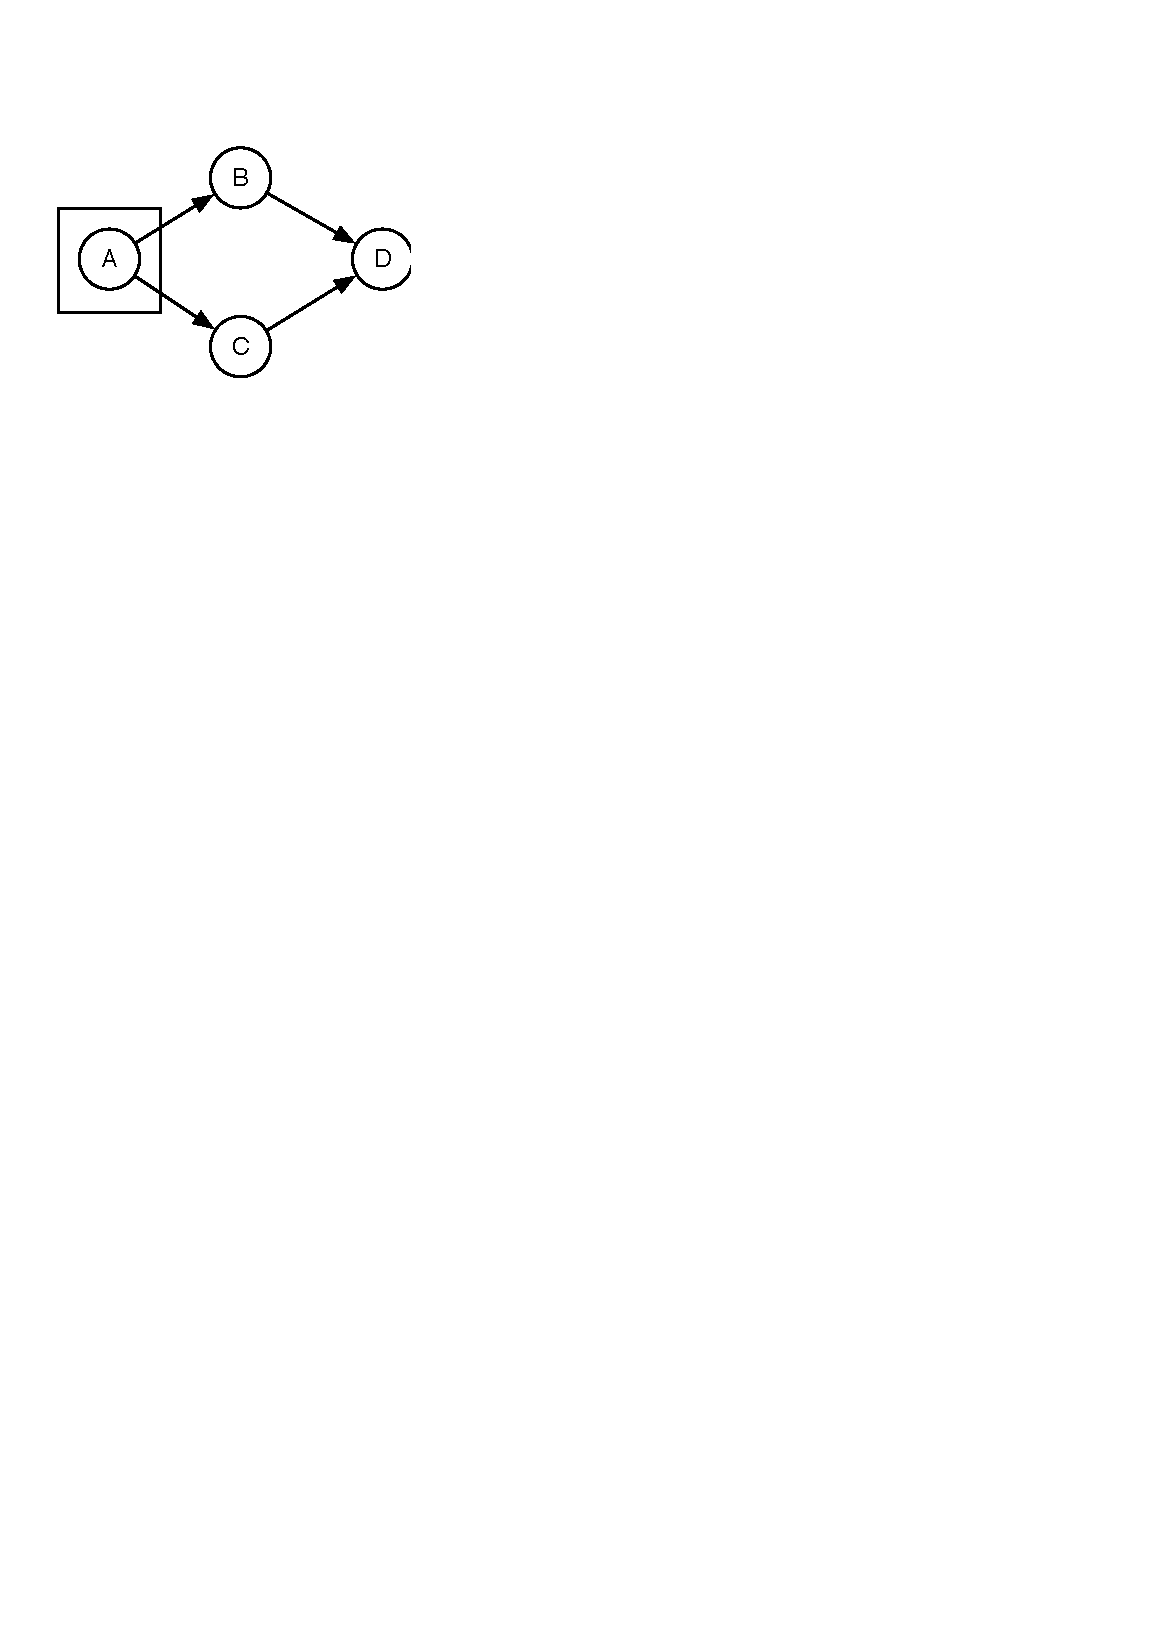
\includegraphics[width=4cm]{images/multi-anchoring}
		\caption{Multi-anchoring.}
		\label{fig:multi-anchoring}
	\end{center}
\end{figure}

\subsection{Cycle in Topology}

Technically it is possible to have cycle in Storm topologies. An infinite cycle of processing would create an infinite tuple tree and make it impossible for Storm to ever acknowledge that spout tuple. Therefore,  tuple trees should terminate at some point.

\begin{figure}[H]
	\begin{center}
		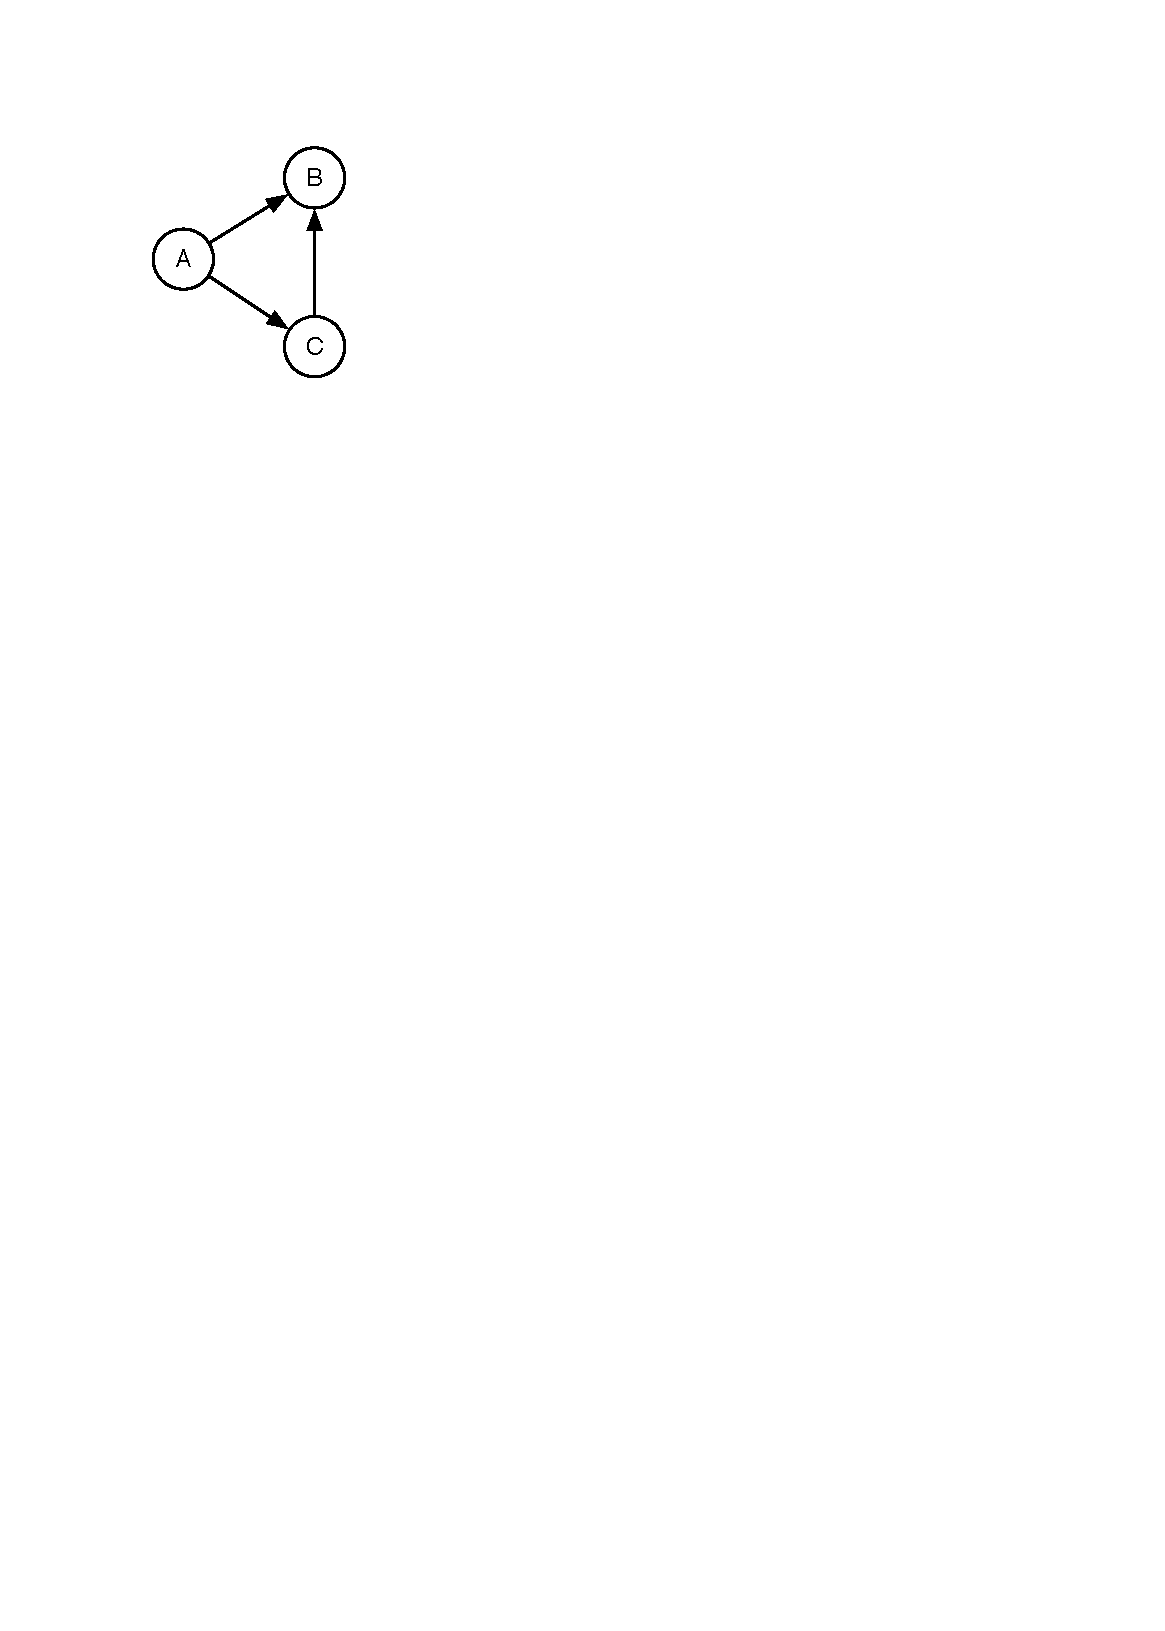
\includegraphics[width=3cm]{images/cycle}
		\caption{Cycle n Topology.}
		\label{fig:cycle}
	\end{center}
\end{figure}

\subsection{Persistent Data}

If two processing elements wants to update a same entity in a storage, there should be a consistency mechanism in place. 


\begin{figure}[H]
	\begin{center}
		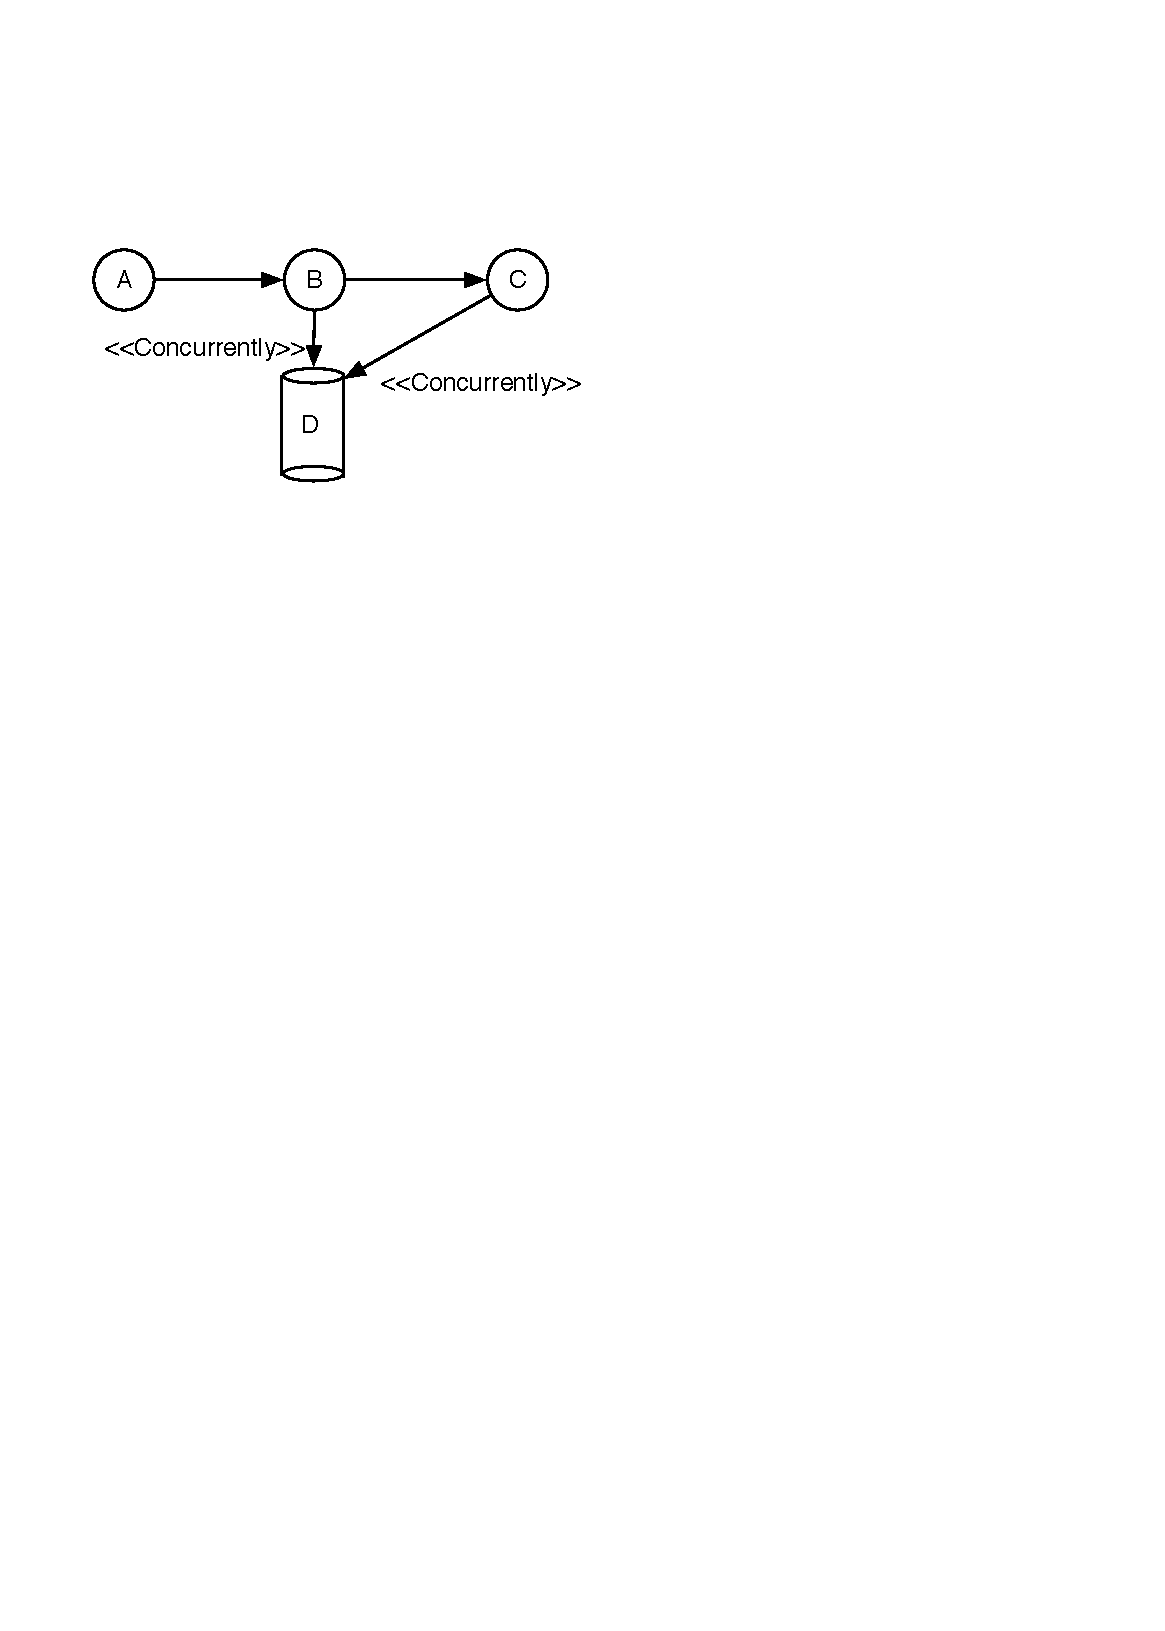
\includegraphics[width=4cm]{images/persistence}
		\caption{Concurrency management.}
		\label{fig:persistence}
	\end{center}
\end{figure}

\section{Algorithmic Analysis on Stream Topologies}

\subsection{fan-in/fan-out}

For Bolts, fan-in is the number of processing elements (Bolts and Spouts) that are connected to this specific bolt in the topology and fan-out is the number of PEs that are dependent to this specific bolt. For Spouts, fan-in is the number of topics (from Kafka) that this specific spout is subscribed to and fan out is the number of bolts that is dependent to this spout.

\begin{figure}[H]
	\begin{center}
		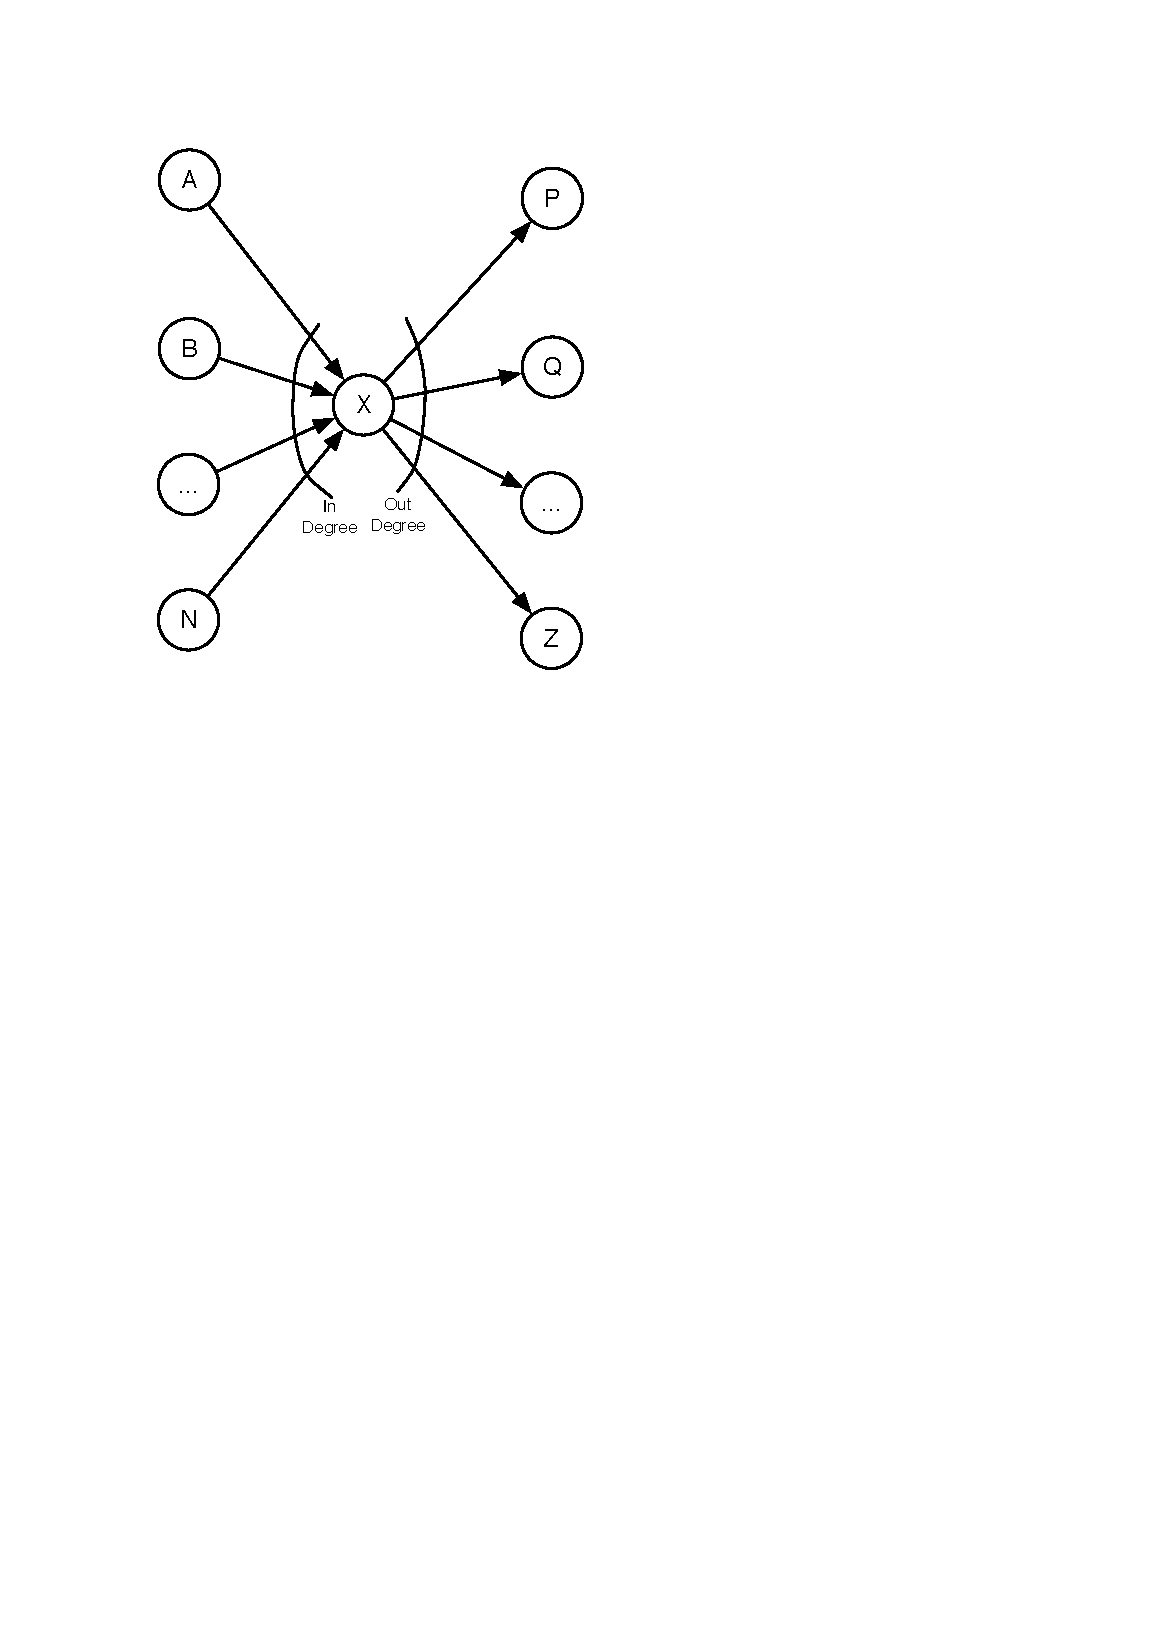
\includegraphics[width=3cm]{images/fan-in-out}
		\caption{Fan-in fan-out in Stream topologies.}
		\label{fig:fan}
	\end{center}
\end{figure}

\subsection{topology cascading}

By topology cascading, we mean connecting two different Storm topologies via a messaging framework like Kafka.

\begin{figure}[H]
	\begin{center}
		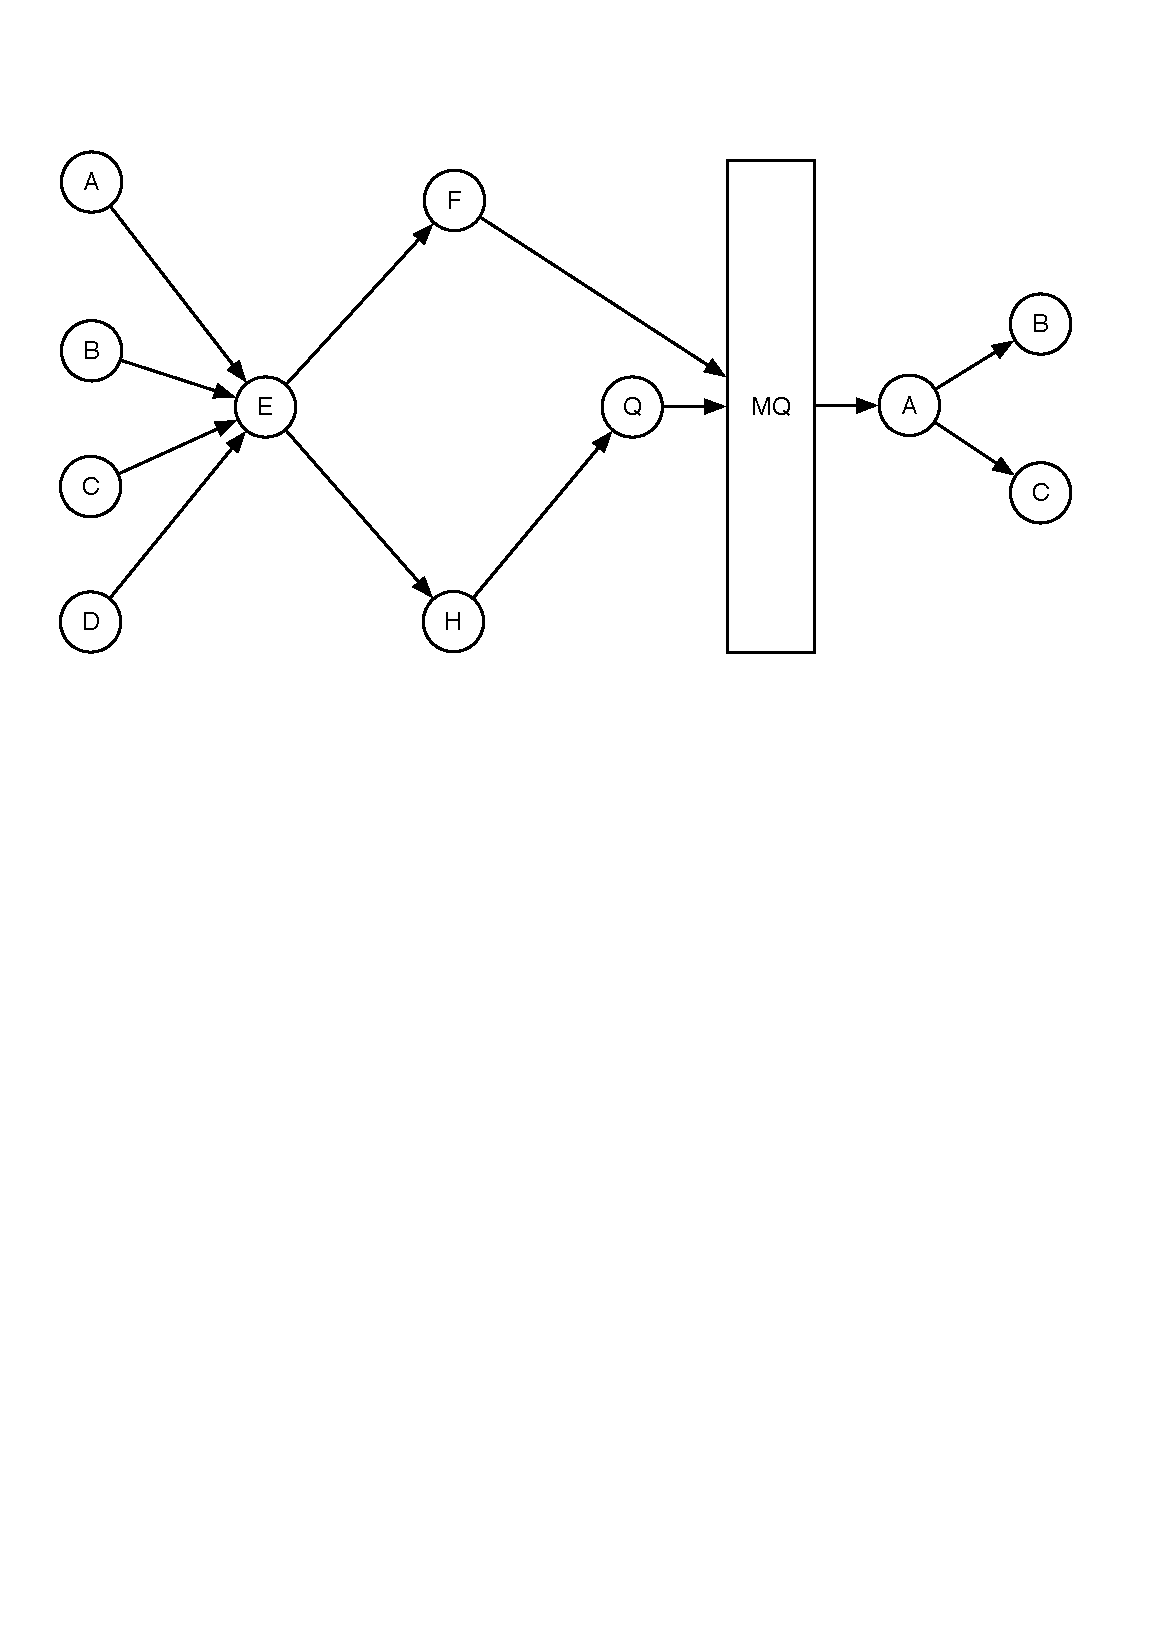
\includegraphics[width=5cm]{images/cascading}
		\caption{cascading.}
		\label{fig:cascading}
	\end{center}
\end{figure}

\subsection{Topology clustering}
Identifying the coupled processing elements and put the in a cluster in a way that elements in a cluster have high cohesion and less coupled with the elements in other clusters.

\begin{figure}[H]
	\begin{center}
		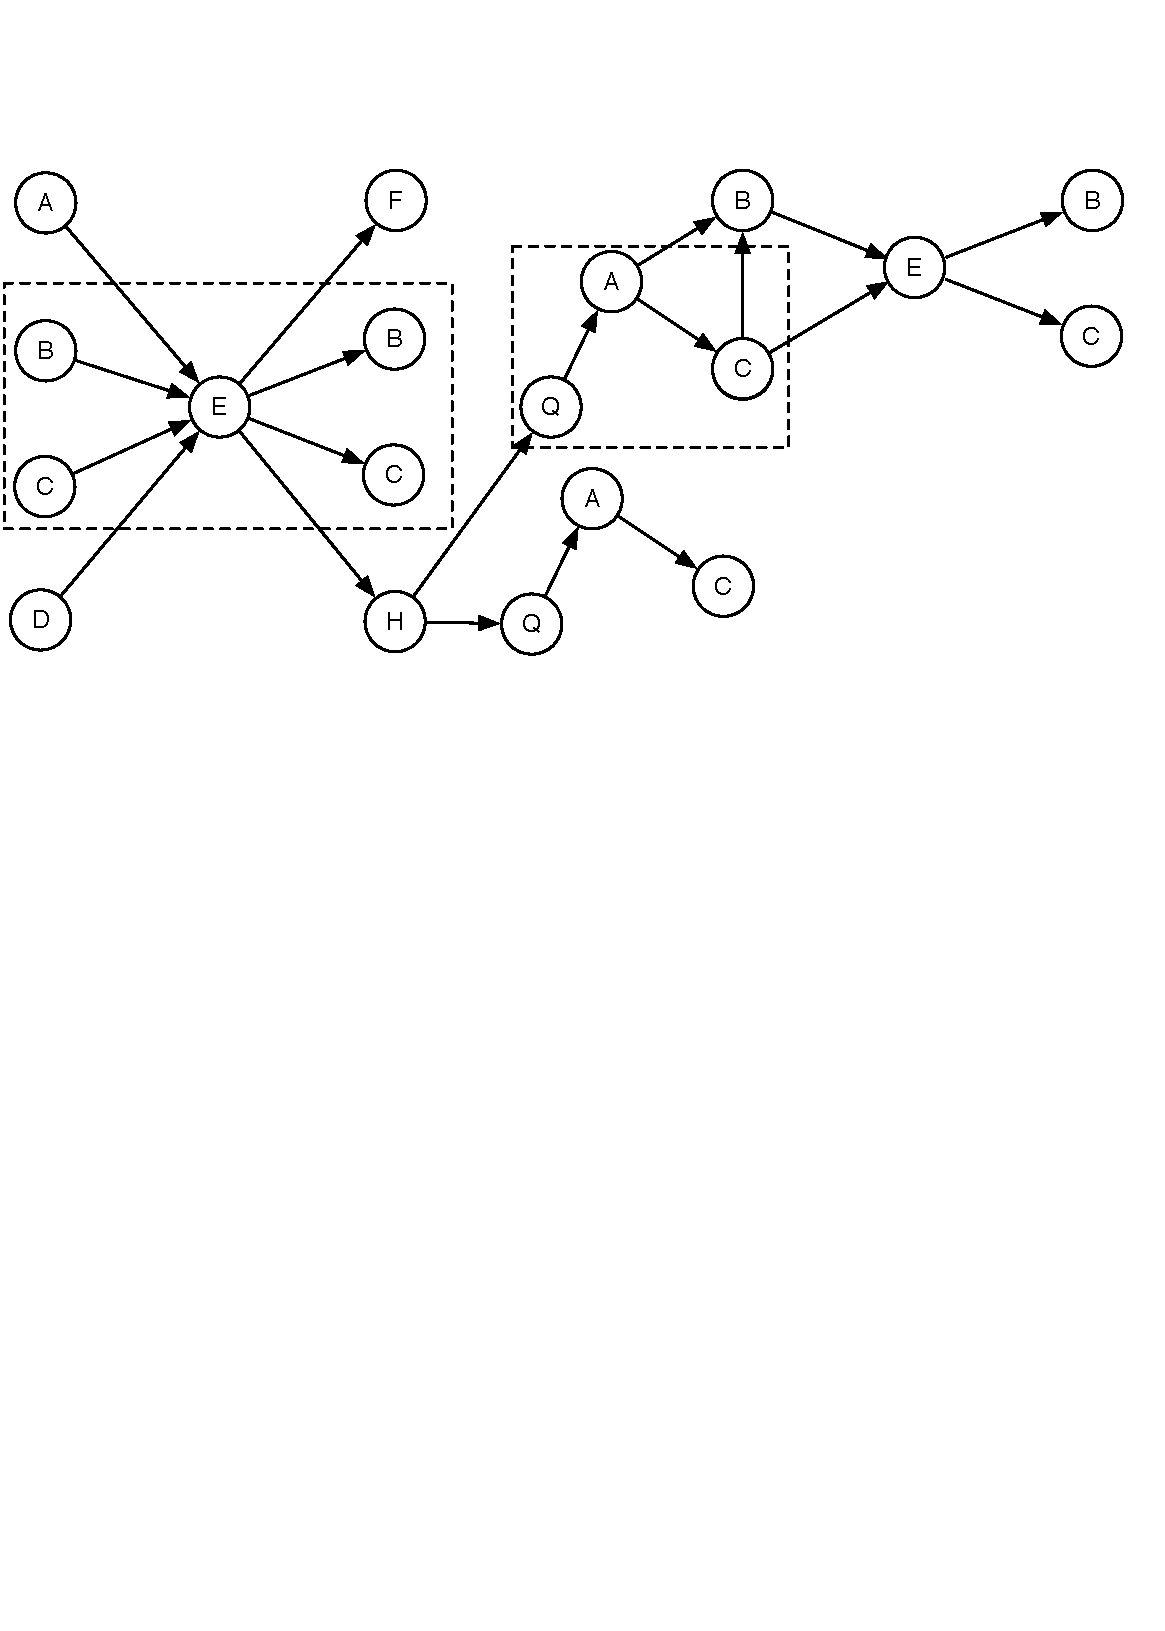
\includegraphics[width=5cm]{images/clustering}
		\caption{clustering.}
		\label{fig:clustering}
	\end{center}
\end{figure}

\subsection{Computation funnel}
When there is not a path from data source (spout) to the bolts that sends out the tuples off the topology to another topology through a messaging framework or through a storage.

\begin{figure}[H]
	\begin{center}
		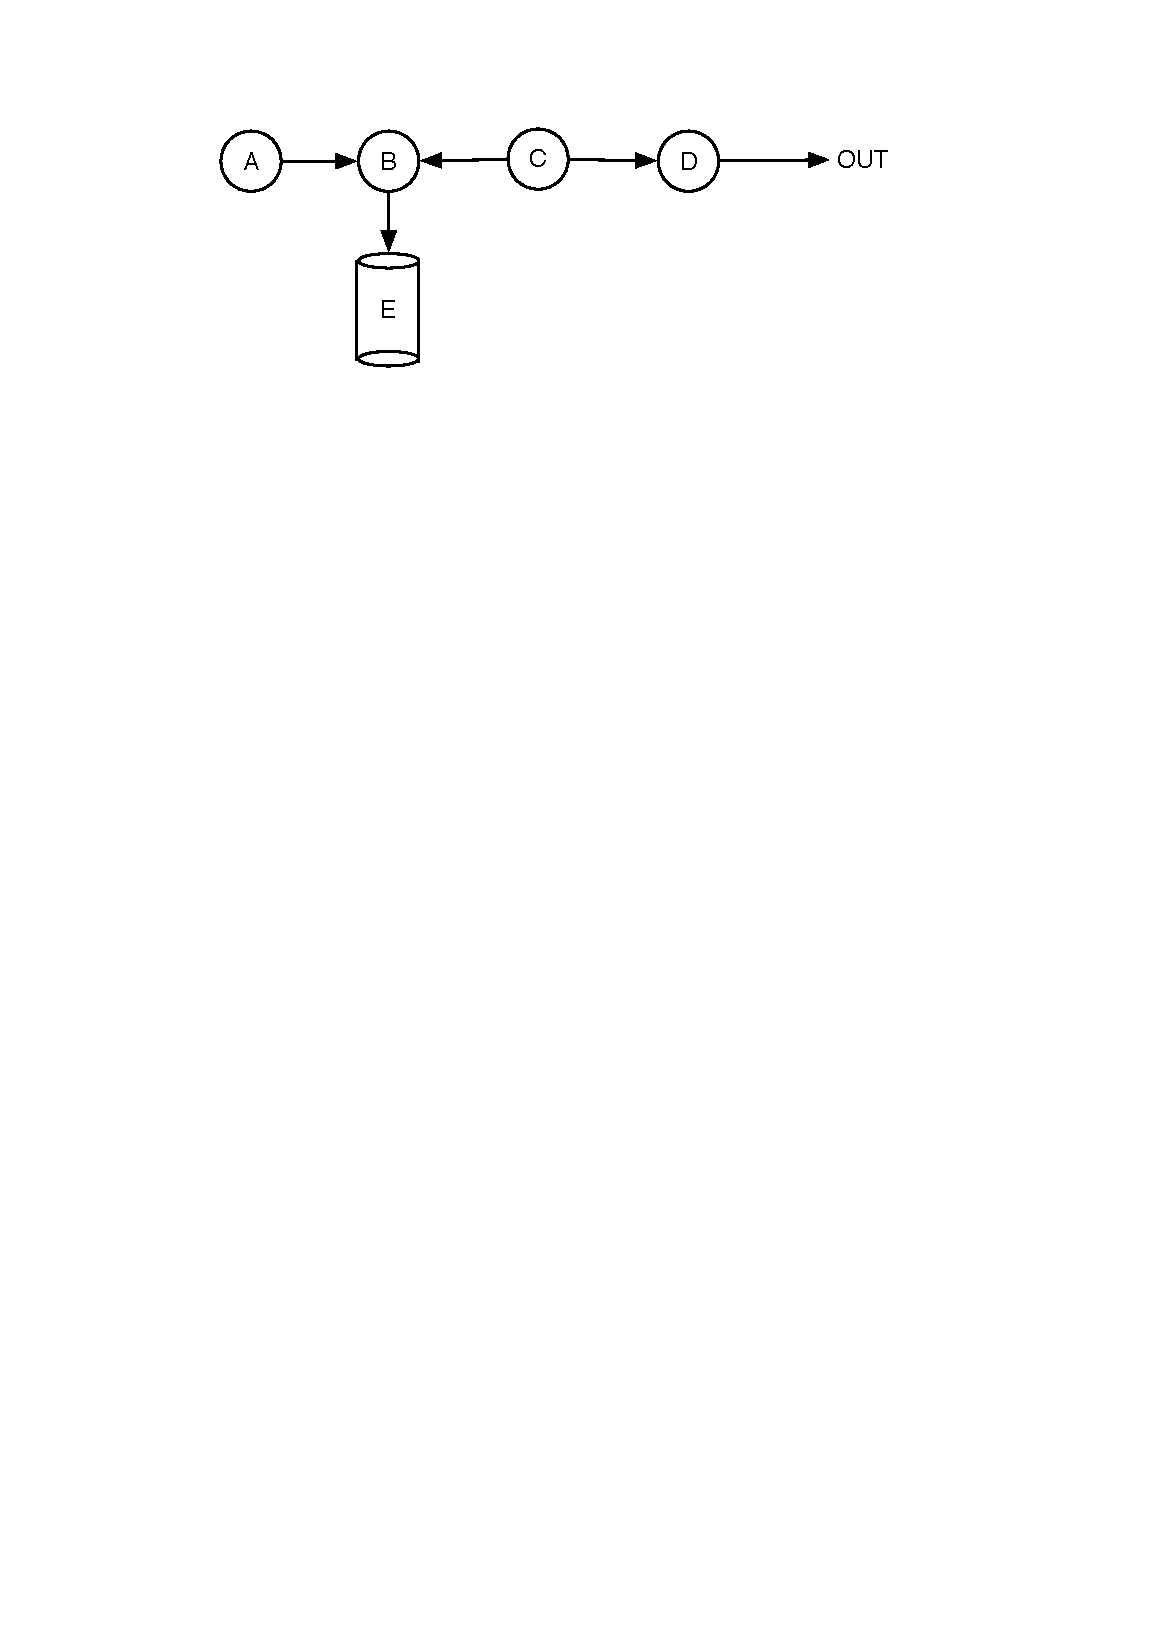
\includegraphics[width=5cm]{images/funnel}
		\caption{funnel.}
		\label{fig:funnel}
	\end{center}
\end{figure}

\subsection{Linearizing a topology}

Sorting the processing elements in a topology in a way that topology looks more linear visually.

\begin{figure}[H]
	\begin{center}
		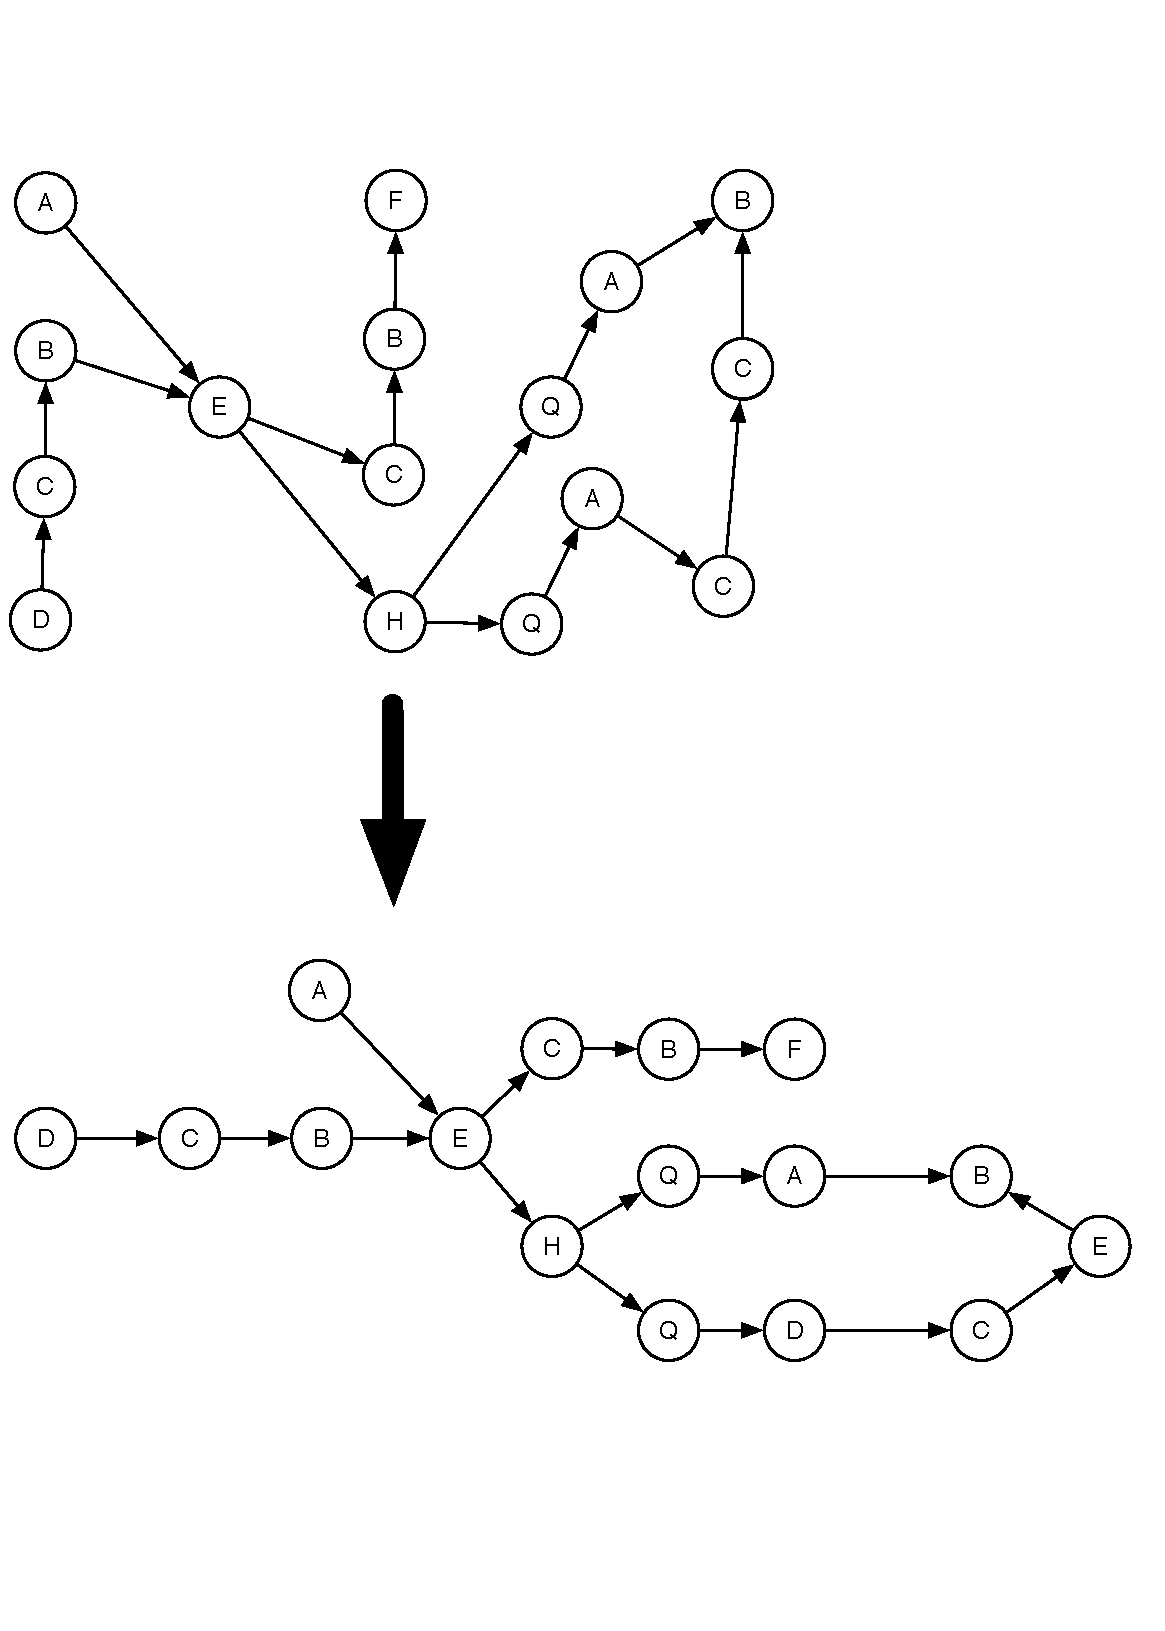
\includegraphics[width=5cm]{images/linearizing}
		\caption{linearizing.}
		\label{fig:linearizing}
	\end{center}
\end{figure}